%----------------------------------------------------------------------------
\appendix
%----------------------------------------------------------------------------
\chapter*{\fuggelek}\addcontentsline{toc}{chapter}{\fuggelek}
\setcounter{chapter}{\appendixnumber}
%\setcounter{equation}{0} % a fofejezet-szamlalo az angol ABC 6. betuje (F) lesz
\numberwithin{equation}{section}
\numberwithin{figure}{section}
\numberwithin{lstlisting}{section}
%\numberwithin{tabular}{section}

%----------------------------------------------------------------------------
\section{A parancssori interfész felülete}
\label{sec:fuggelek}
%----------------------------------------------------------------------------
\begin{figure}[!ht]
	\label{fig:cli_1cc}
	\centering
	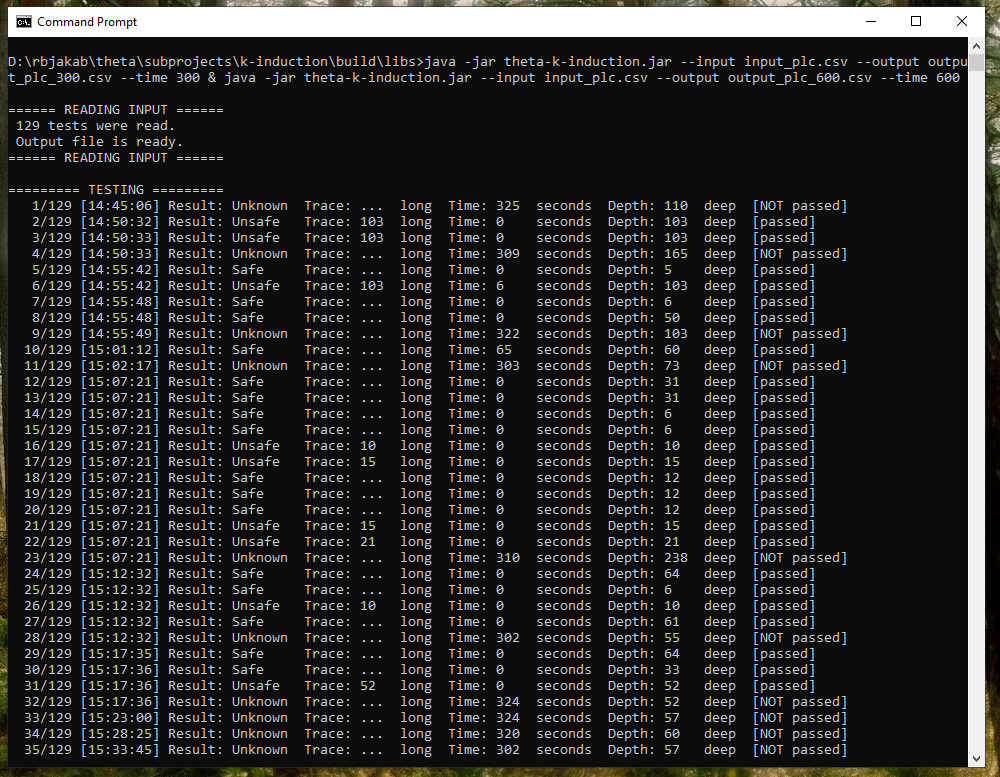
\includegraphics[width=135mm, keepaspectratio]{figures/cli/eleje.png}
	\caption{A parancssori interfész a futás elején.} 
\end{figure}

\begin{figure}[!ht]
	\label{fig:cli_2bb}
	\centering
	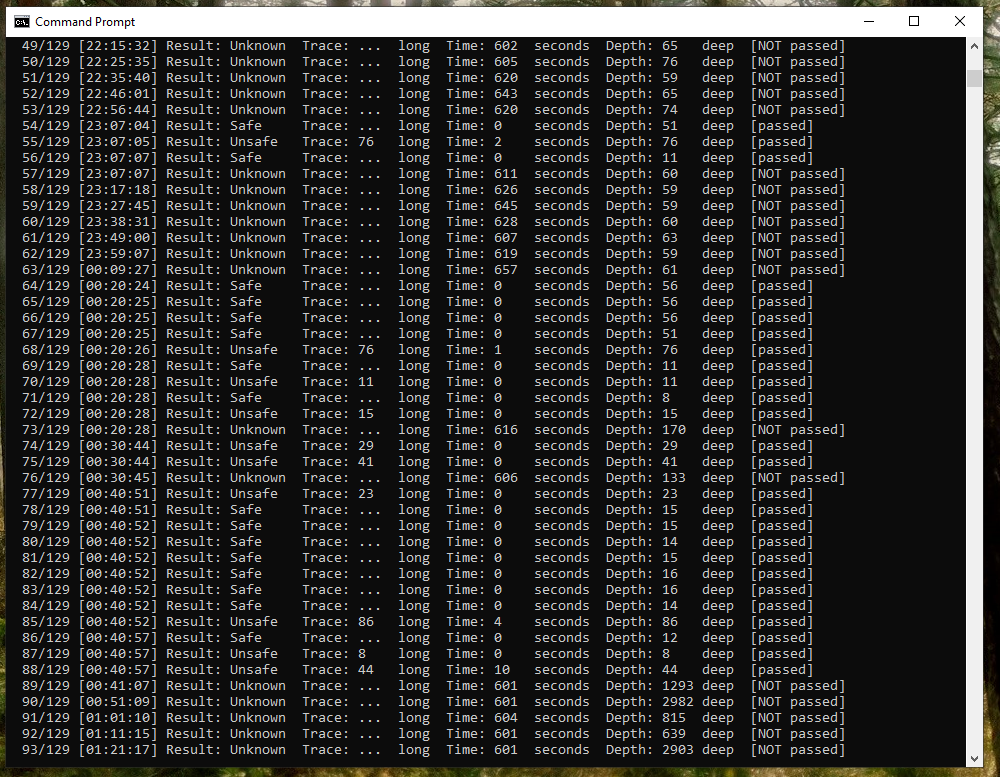
\includegraphics[width=135mm, keepaspectratio]{figures/cli/kozepe.png}
	\caption{A parancssori interfész futás közben.} 
\end{figure}

\begin{figure}[!ht]
	\centering
	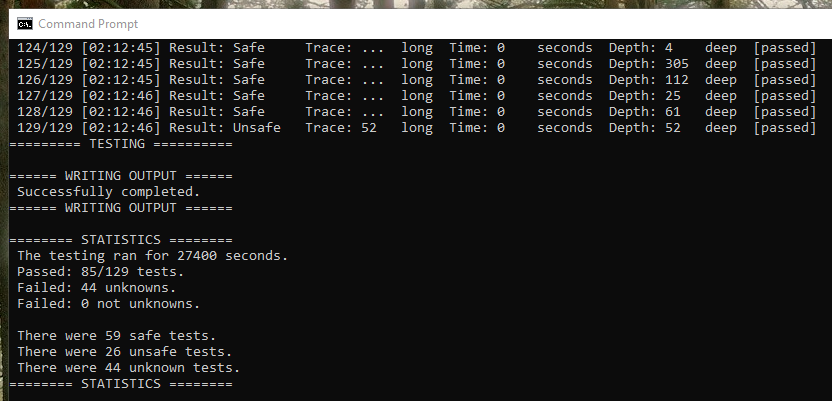
\includegraphics[width=135mm, keepaspectratio]{figures/cli/vege.png}
	\caption{A parancssori interfész a futás végén.\label{fig:cli_3}} 
\end{figure}